\appendix

%%%%%%%%%%%%%%%%%%%%%%%%%%%%%%%%%%%%%%%%%%%%%%%%%%%%%%%%%%%%%%%%%%%%%%%%%%%%%%%%%%%%%%%%%%%%%%%%%
%
%
%
%%%%%%%%%%%%%%%%%%%%%%%%%%%%%%%%%%%%%%%%%%%%%%%%%%%%%%%%%%%%%%%%%%%%%%%%%%%%%%%%%%%%%%%%%%%%%%%%%
\clearpage
\onecolumngrid
\section{Supplementary Figures}
\setcounter{figure}{0}
\renewcommand{\thefigure}{SF\arabic{figure}}



% --------------- Dim red time series and free energy profiles
\begin{figure}[h!]
    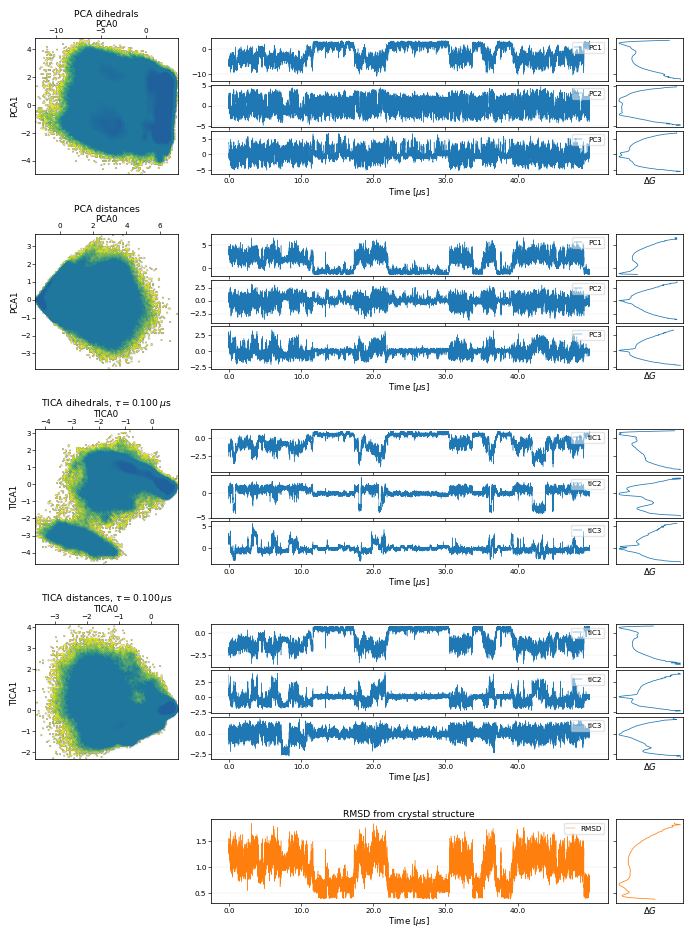
\includegraphics[width=0.7\linewidth]{figures/dimred_figure.png}
\caption{\small
Comparison of the compressed trajectory representations obtained from the four feature--dimensionality-reduction pipelines. 
Rows correspond to PCA dihedrals, PCA contact distances, TICA dihedrals, and TICA contact distances. 
The left column shows the projection onto the first two reduced coordinates. 
The right block shows, for each pipeline, the time series of the first three reduced coordinates over the first $40\,\mu\mathrm{s}$, together with the corresponding one-dimensional free-energy profiles computed from the full trajectory. 
The bottom row reports the RMSD from the crystal structure and its one-dimensional free-energy profile as a reference folding coordinate. 
The PCA projections show mostly unimodal one-dimensional free-energy profiles and less pronounced residence-and-jump behavior with respect to the tICA representations. 
}
    \label{suppfig:dimred_figure}
\end{figure}


% --------------- MSM connectivity and active population as a function of lag time
\begin{figure}[h!]
    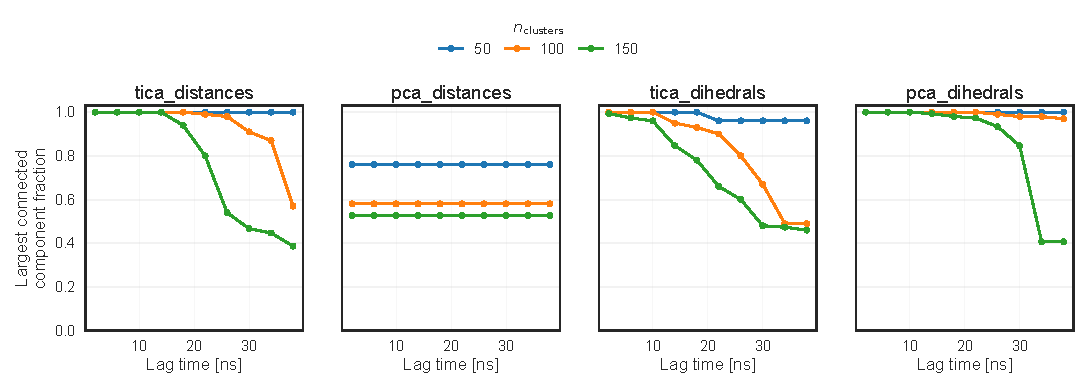
\includegraphics[width=0.7\linewidth]{figures/largest_connected_component_vs_lag.pdf}
    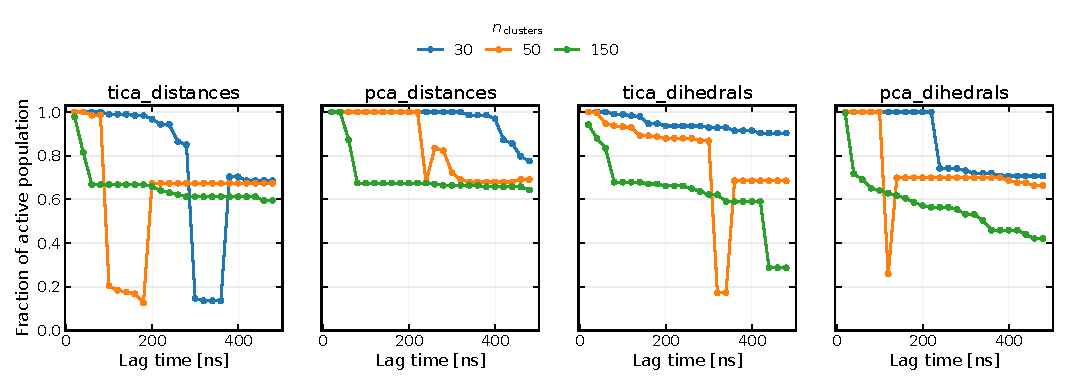
\includegraphics[width=0.7\linewidth]{figures/active_population_vs_lag.pdf}
    \caption{\small \textbf{MSM connectivity and active population as a function of lag time.}
    Top panel: fraction of microstates in the largest connected component of the MSM as a function of lag time. 
    Bottom panel: fraction of the total equilibrium population contained in the largest connected component of the MSM as a function of lag time}
    \label{suppfig:largest_connected_component_vs_lag}
\end{figure}



% ------------- First eigenvector of all models -------------------------
\begin{figure}[!t]
    \centering
    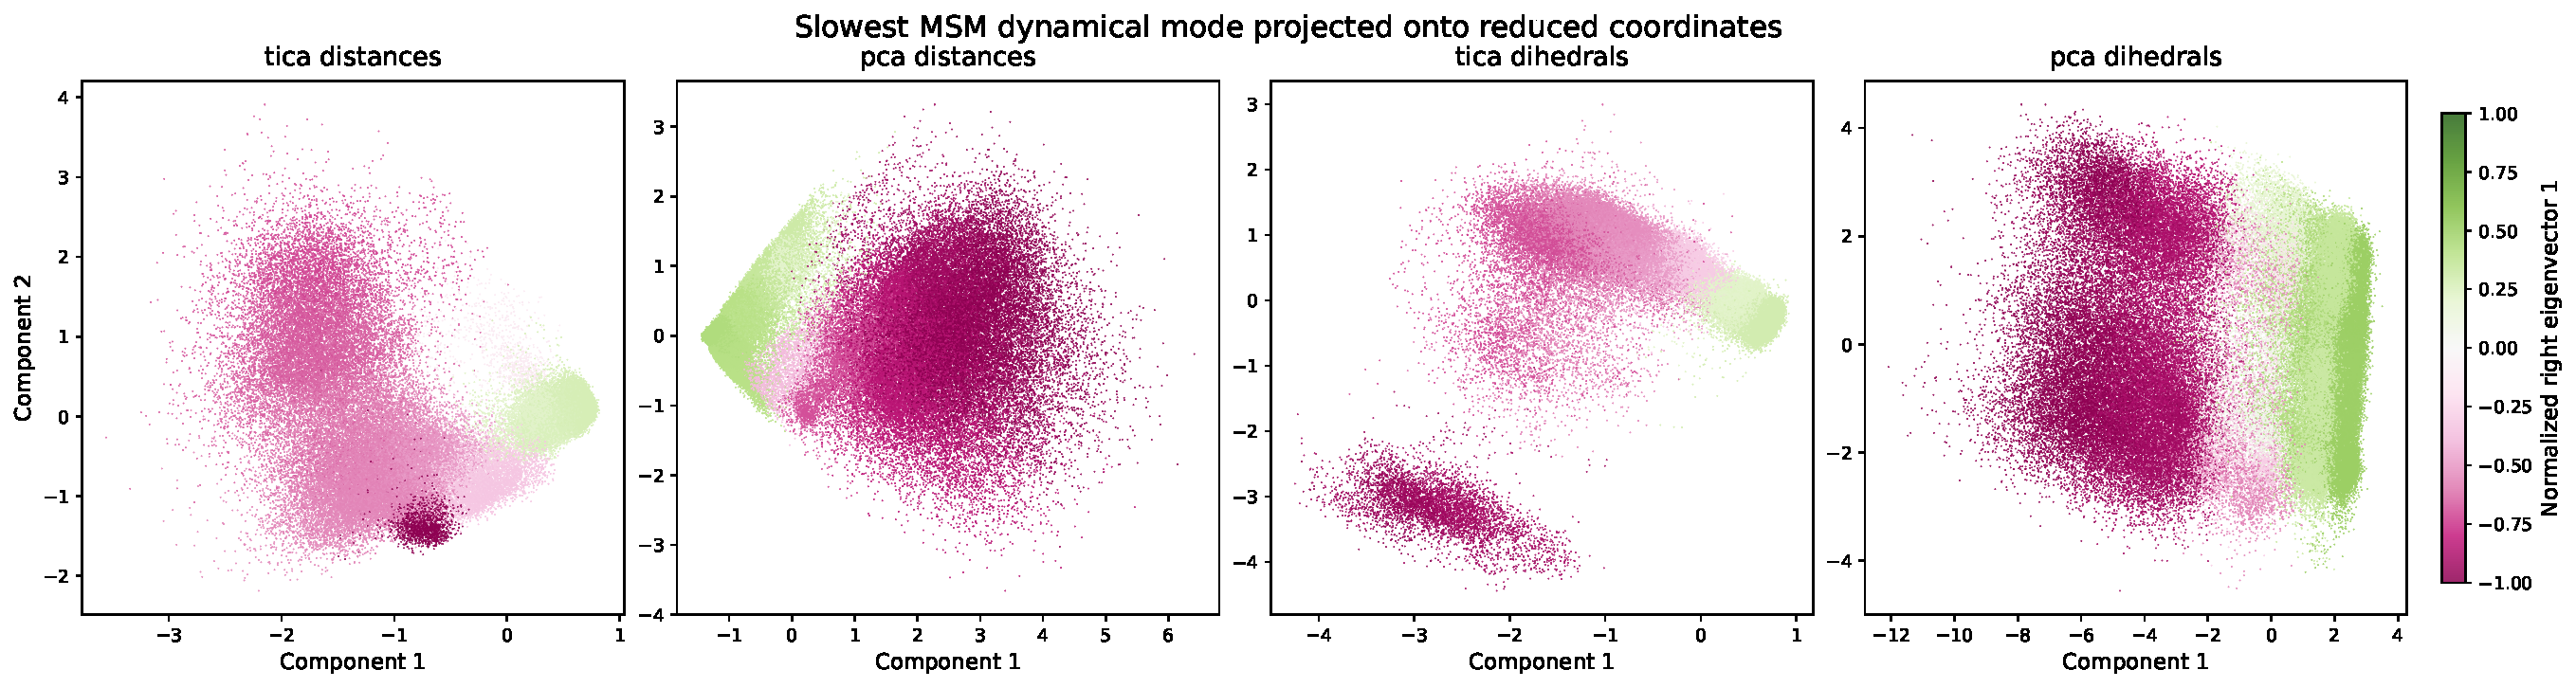
\includegraphics[width=0.8\linewidth]{figures/msm_right_eigenvector_1_projection.pdf}
    \vspace{1em}
    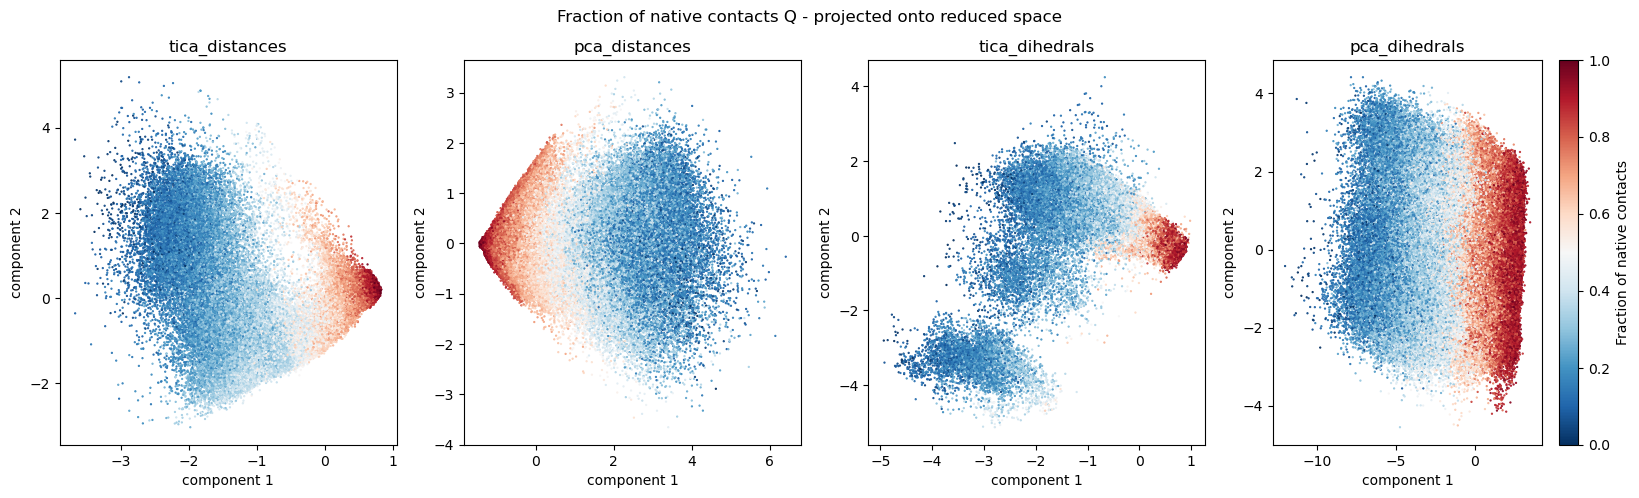
\includegraphics[width=0.8\linewidth]{figures/Q_reduced_projection.png}
    \caption{\footnotesize \textbf{Comparison between the slowest MSM relaxation mode and a structural folding descriptor.} 
    Top row: values of the first non-trivial eigenvector projected onto the first two components of the reduced coordinate space.
    Positive and negative components identify regions that exchange probability on the slowest resolved timescale of the Markov model. 
    Bottom row: projection of the fraction of native contacts, Q, onto the same coordinates. 
    The close correspondence between the eigenvector sign pattern and the distribution of $Q$ indicates that the slowest kinetic process 
    captured by the MSM is associated with the folding-unfolding transition.}
    \label{fig:eigenvectors}
\end{figure}



\begin{figure}[h!]
    \centering
    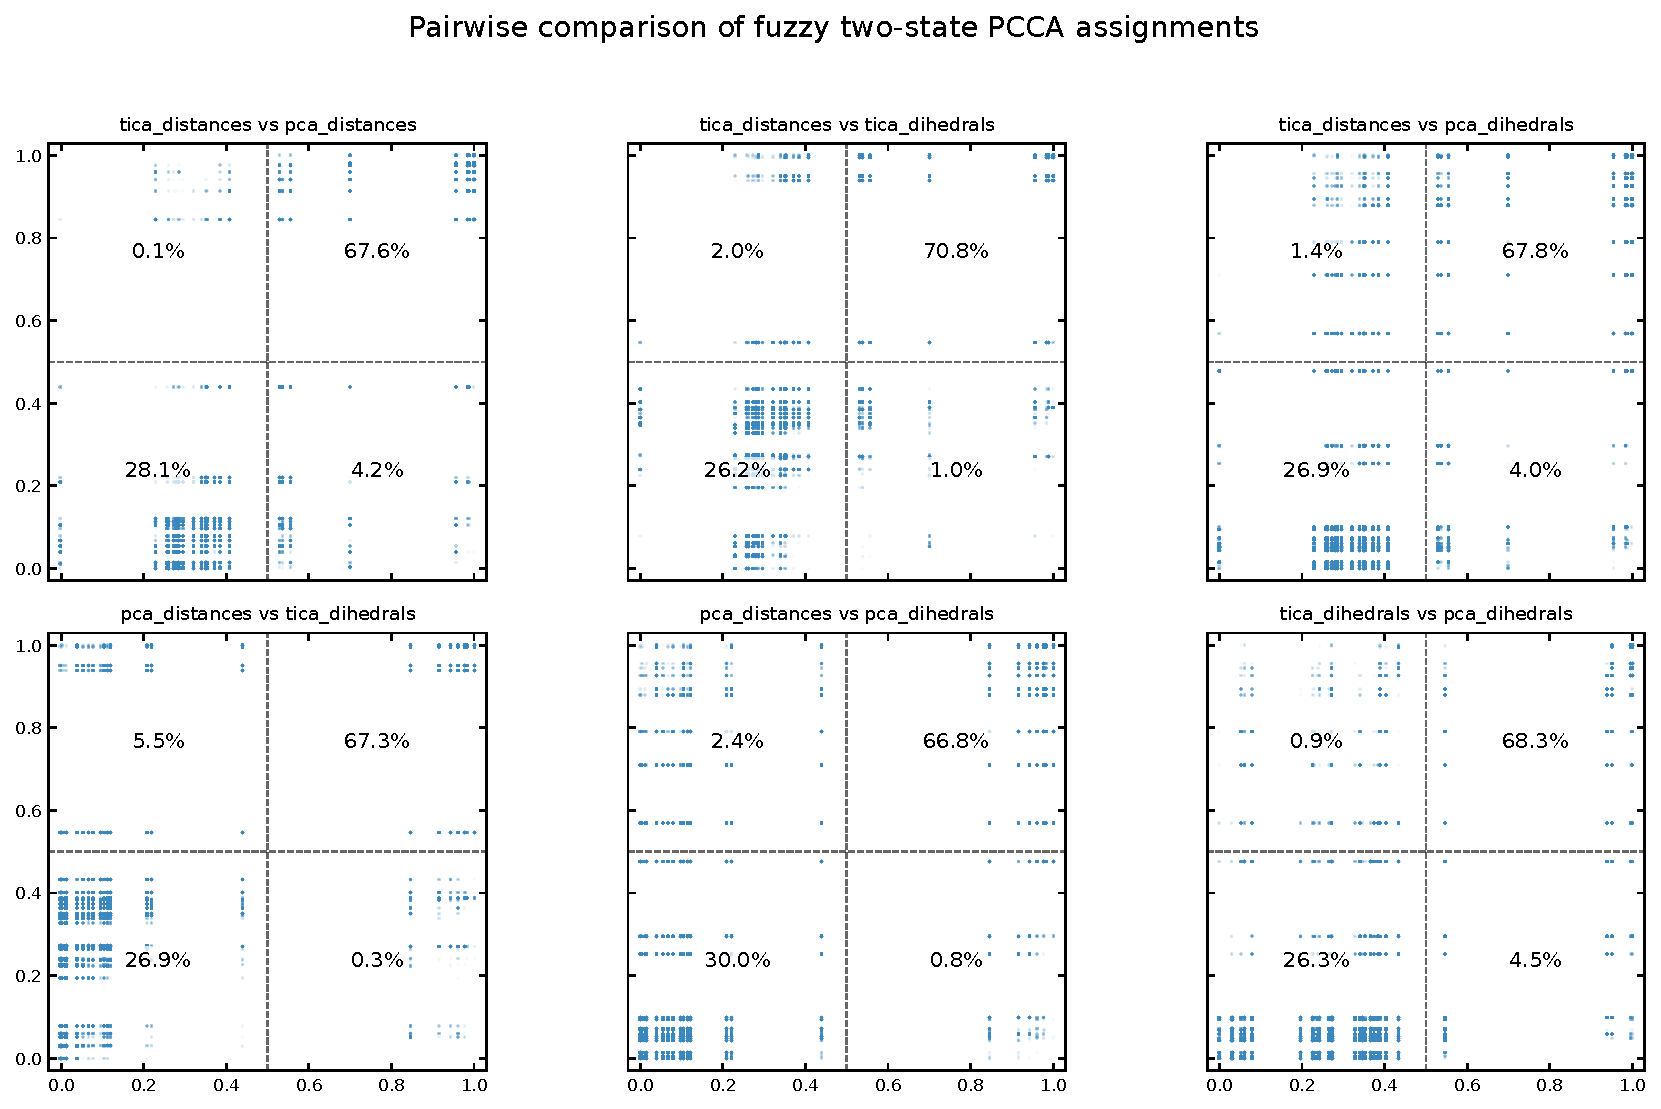
\includegraphics[width=0.8\linewidth]{figures/pairwise_pcca_membership_scatter_quadrants_report.pdf}
    \caption{\small \textbf{Fuzzy membership probabilities of the trajectory frames to the two macrostates across models.} Each panel shows the fuzzy membership probability of each frame in the trajectory to macrostate $0$ (denatured basin) and macrostate $1$ (native basin) for a different model. The models based on distances (tica-distances and pca-distances) show very similar distributions, while the tica-dihedrals model exhibits a broader distribution, particularly for frames assigned to the denatured basin. This indicates that the tica-dihedrals model has more uncertainty in assigning frames to the denatured basin.}
    \label{suppfig:fuzzy_memberships_models}
\end{figure}

\begin{table}[h!]
\caption{Pairwise correlations between frame-wise PCCA membership probabilities for the folded basin. Pearson correlations quantify linear agreement, whereas Spearman correlations quantify agreement in the rank ordering of frames along the folded-basin membership coordinate.}
\label{supptab:two_state_model_correlation}
\begin{tabular}{lcc}
\hline
Model pair & Pearson & Spearman \\
\hline
tICA distances -- PCA distances & 0.990 & 0.911 \\
tICA distances -- tICA dihedrals & 0.923 & 0.826 \\
tICA distances -- PCA dihedrals & 0.876 & 0.831 \\
PCA distances -- tICA dihedrals & 0.910 & 0.821 \\
PCA distances -- PCA dihedrals & 0.876 & 0.847 \\
tICA dihedrals -- PCA dihedrals & 0.885 & 0.930 \\
\hline
\end{tabular}
\end{table}


\begin{figure}[h!]
    \centering
    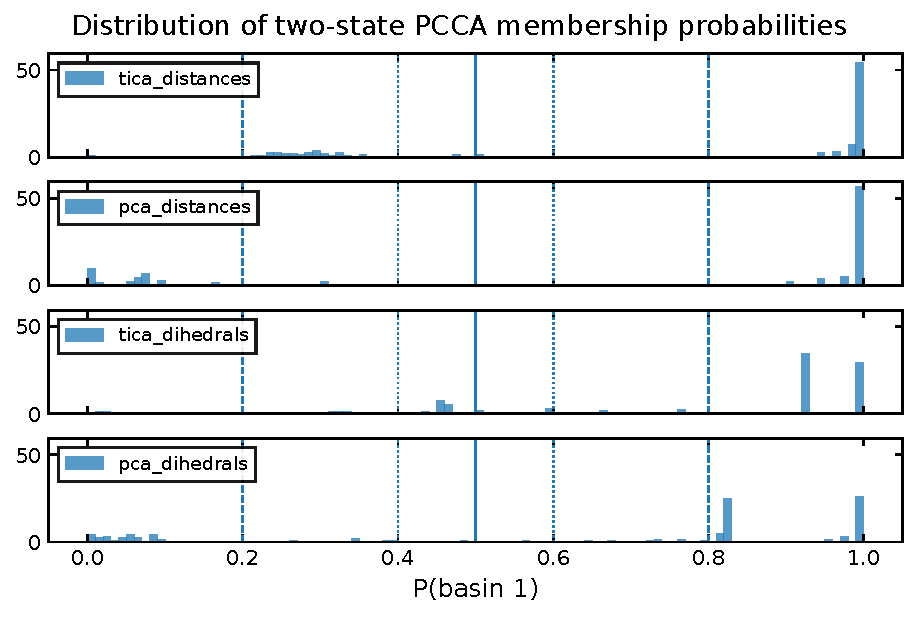
\includegraphics[width=0.4\linewidth]{figures/pcca_membership_probability_distributions.pdf}
    \caption{\small the distributions of fuzzy membership probabilities assigned to frames, for basin $1$ across the four models. }
    \label{suppfig:pcca_frames_prob_density}
\end{figure}

% ------------- Second eigenvector of tica models only -------------------------
\begin{figure}[!t]
    \centering
    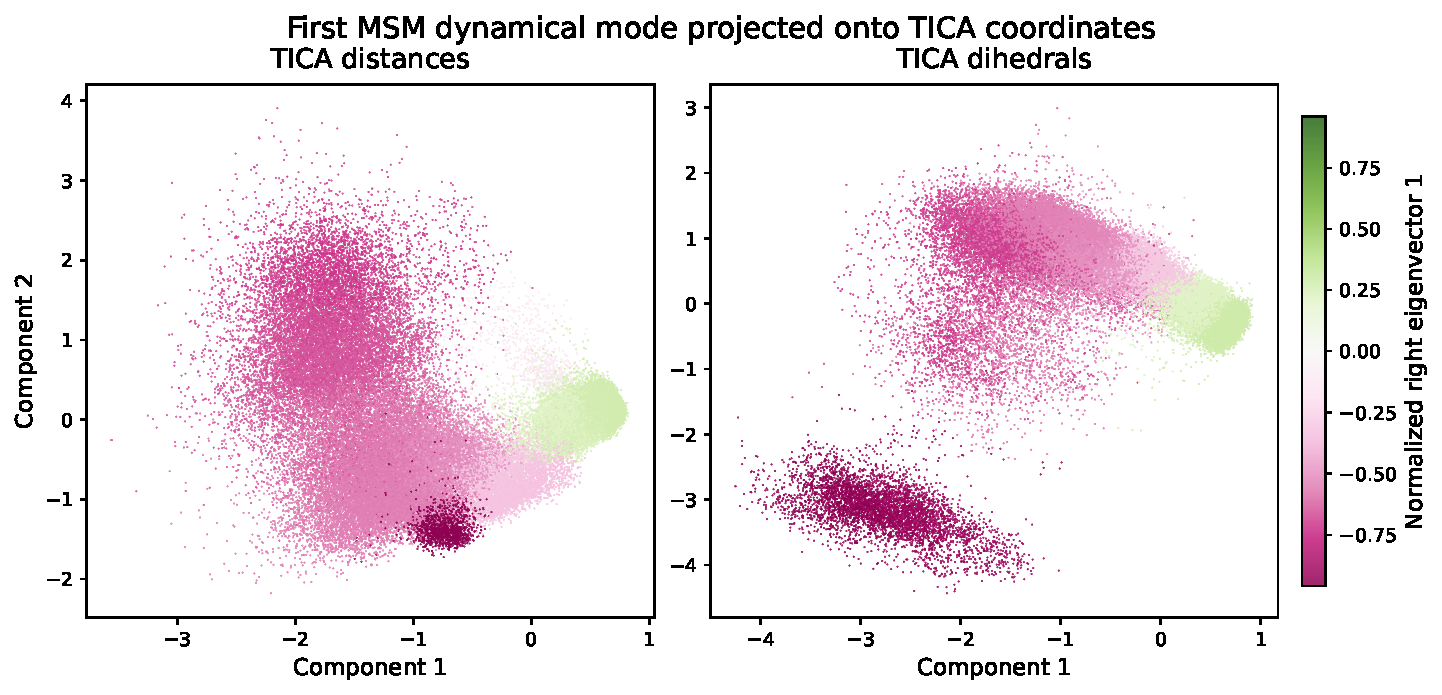
\includegraphics[width=0.45\linewidth]{figures/tica_right_eigenvector_1_projection.pdf}
    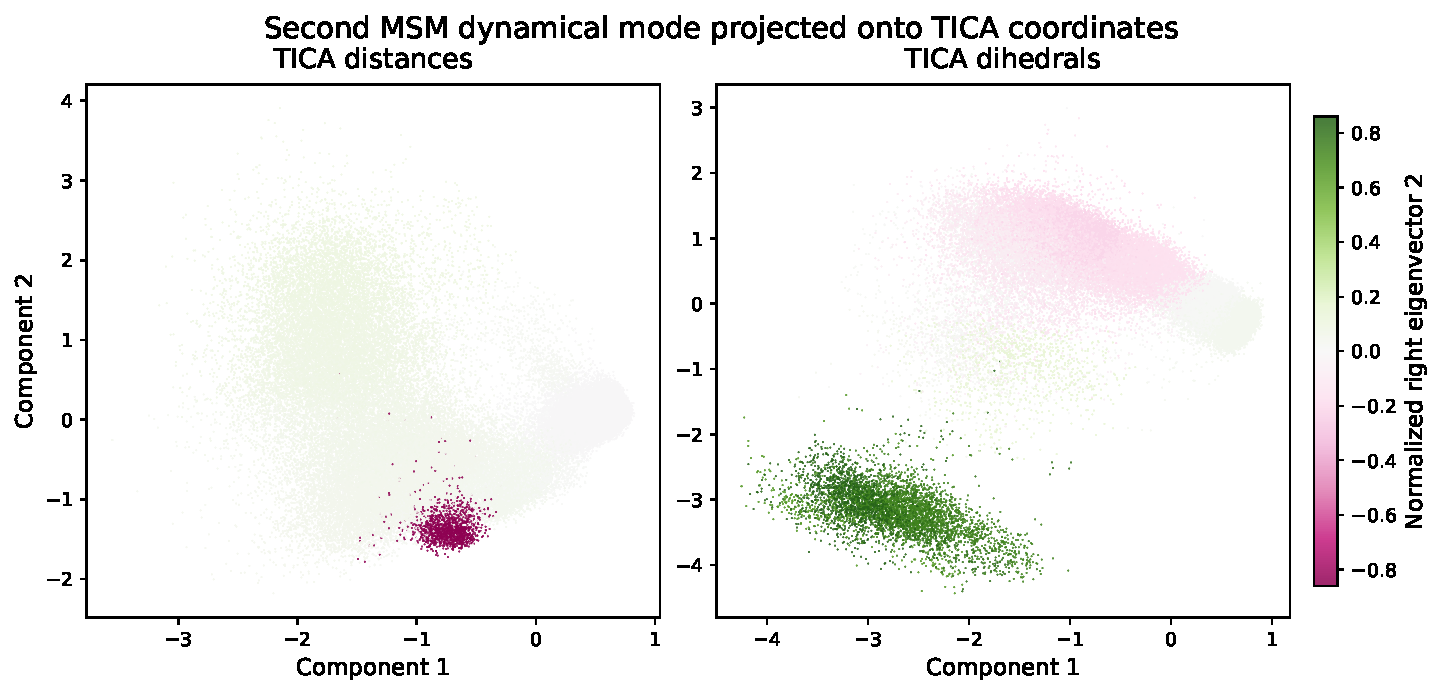
\includegraphics[width=0.45\linewidth]{figures/tica_right_eigenvector_2_projection.pdf}
    \vspace{1em}
    \caption{\footnotesize {First two non-trivial eigenvectors of the tICA-based MSMs projected onto the first two tICA coordinates.}}
    \label{fig:tica_second_eigvec}
\end{figure}





